\section{Methoden}

Das Projekt \textit{DeepXRay} hat ein klares Ziel (siehe \secref{sec:projektauftrag}): Auf Basis bestehender Machine-Learning-Modelle soll ein Prototyp für einen Webservice erstellt werden, der sich später in andere Anwendungen integrieren lässt. Ein \textit{rein} agiles Vorgehen ist somit für das Projekt nicht geeignet.

Die Ausgangslage des Projekts zu verstehen, und die zur Verfügung gestellten Artefakte verwenden zu können, ist ein wichtiger Teil des Projekts. An die Integration der einzelnen Teile kann erst gedacht werden, wenn deren Funktionsweise verstanden ist. Eine reine Top-Down-Planung wie im V-Modell oder im Wasserfallmodell ist somit nicht praktikabel.

Ein hybrides Modell, bei dem das übergeordnete Ziel (lauffähiger Prototyp für Webservice) von Anfang an bekannt ist, die einzelnen Aufgabenblöcke aber erst detailliert geplant werden, wenn deren Voraussetzungen geschaffen worden sind, ist somit besser geeignet.

\subsection{Projektphasen}
\label{sec:projektphasen}

Das Projekt soll in den folgenden drei Phasen umgesetzt werden:

\begin{description}
    \item[Erste Phase (Modelle)] Die bestehenden Machine-Learning-Modelle ‒ drei an der Zahl ‒ sind schon etwas älter und basieren auf verschiedenen Technologien. Die Modelle müssen wieder lauffähig gemacht werden, sodass man sie für das Erstellen von Predictions verwenden kann. Die Inputs und Outputs der Modelle müssen dabei verstanden und dokumentiert werden, damit die nächste Phase in Angriff genommen werden kann.
    \item[Zweite Phase (Architektur)] Der zu erstellende Webservice-Prototyp hat einerseits eine externe Schnittstelle, die zu einem späteren Zeitpunkt von anderen Applikationen angesteuert werden können muss, und andererseits interne Schnittstellen, um die Machine-Learning-Modelle zu koordinieren. Beide Schnittstellen müssen definiert werden. Hierbei kann die Gestaltung der internen Schnittstellen einerseits durch die bestehenden Artefakte und andererseits durch die gewählte externe Schnittstelle beeinflusst werden. Am Ende der zweiten Phase soll auf Basis der besprochenen Architekturansätze ein Architekturentscheid gefällt werden.
\item[Dritte Phase (Orchestrierung)] Auf Basis der lauffähigen Modelle und der entworfenen Architektur sollen nun die einzelnen Komponenten orchestriert werden, sodass sie gegen aussen als ein System ansprechbar sind. Der Prototyp ist auf einer für Demo- und Testzwecke geeigneten Umgebung ausführbar. Für die Anwendung als ganzes sowie für deren einzelne Komponenten gibt es automatisierte Testfälle. Weiter wird eine weitgehend automatisierte Evaluation benötigt, womit die Qualität des Systems eingeschätzt ‒ und später mit verbesserten Versionen des Systems verglichen werden kann.
\end{description}

Da die Aufgaben und die Struktur der einzelnen Phasen jeweils von den Ergebnissen der vorherigen Phasen abhängig sind, kann immer nur zum Ende der einen Phase die nächste Phase geplant werden. Dieses Kapitel wird deshalb im Projektverlauf laufend ergänzt. Das Ende einer jeden Phase ist sogleich ein Meilsenstein, für welchen Ziele, Artefakte und Termine zu definieren sind. Am Ende jeder Projektphase wird diese im Bezug auf Risiken und die Zielerreichung reflektiert.

Die Projektplanung beschränkt sich dabei auf das zu erstellende Software-Artefakt: den Webservice-Prototyp. Dokumentationsaufgaben fliessen dabei nur in die Projektplanung ein, wenn eine spätere Projektphase von deren Ergebnis abhängt. Dies ist etwa bei der Dokumentation der Modelle (Inputs/Outputs) und den Architekturvarianten der Fall.  Die drei anderen verlangten Artefakte ‒ Bericht, Web-Abstract und Video ‒ werden im Verlauf des Projekts erstellt und höchstens in der Wochenplanung berücksichtigt, tauchen aber nicht im Abhängigkeitsbaum der einzelnen Phasenpläne auf.

Die einzelnen Aufgaben und Unteraufgaben sollen nicht weiter in Arbeitspakete heruntergebrochen oder zeitlich (Aufwand und Zeitpunkt) eingeplant werden, zumal der zeitliche Rahmen und die Grösse der Aufgabe für ein Projekt, das von einer einzelnen Person umgesetzt wird, problemlos überblickt werden kann. Die vorliegende Projektplanung soll v.a. zur Erkennung der Abhängigkeiten und zum Handhaben der Risiken dienen ‒ nicht für eine detaillierte Arbeitsplanung.

\subsubsection{Erste Phase: Modelle}

\begin{itemize}
    \item \textbf{Ziel:} ausführbare Modelle mit dokumentierter Schnittstelle
    \item \textbf{Artefakte}
        \begin{enumerate}
            \item Modelldaten, Ausführungscode und Laufzeitumgebung für jedes Modell
            \item Dokumentation der Inputs und Outputs
            \item Planung Phase 2
        \end{enumerate}
    \item \textbf{Aufgaben}
        \begin{enumerate}
            \item Modell \texttt{body\_part}
                \begin{multicols}{2}
                    \begin{enumerate}
                        \item Laufzeitumgebung
                        \item Code für Prediction
                        \item Dokumentation
                    \end{enumerate}
                \end{multicols}
            \item Modell \texttt{joint\_extraction}
                \begin{multicols}{2}
                    \begin{enumerate}
                        \item Laufzeitumgebung
                        \item Code für Prediction
                        \item Dokumentation
                    \end{enumerate}
                \end{multicols}
            \item Modell \texttt{ratingen\_score}
                \begin{multicols}{2}
                    \begin{enumerate}
                        \item Modelldaten
                        \item Laufzeitumgebung
                        \item Code für Prediction
                        \item Dokumentation
                    \end{enumerate}
                \end{multicols}
            \item Planung der zweiten Phase
        \end{enumerate}
    \item \textbf{Risiken und Mitigationen}
        \begin{enumerate}
            \item Modell \texttt{ratingen\_score} kann nicht rechtzeitig fertiggestellt werden.
                \begin{enumerate}
                    \item Die Arbeiten werden in Phase 2 fortgeführt.
                    \item Das Modell wird durch ein Dummy-Modell simuliert.
                \end{enumerate}
            \item Die Modelle erstellen unbrauchbare Predictions.
                \begin{enumerate}
                    \item Das Risiko muss getragen werden, zumal die Performance der Modelle nicht Bestandteil der Arbeit ist.
                \end{enumerate}
            \item Die Modelle haben eine schlechte Laufzeitperformance.
                \begin{enumerate}
                    \item Architektonische Massnahmen (z.B. Parallelisierung) zur Erhöhung der Performance werden ergriffen.
                    \item Eine geeignete Laufzeitumgebung wird gewählt.
                \end{enumerate}
        \end{enumerate}
\end{itemize}

\begin{figure}
    \centering
    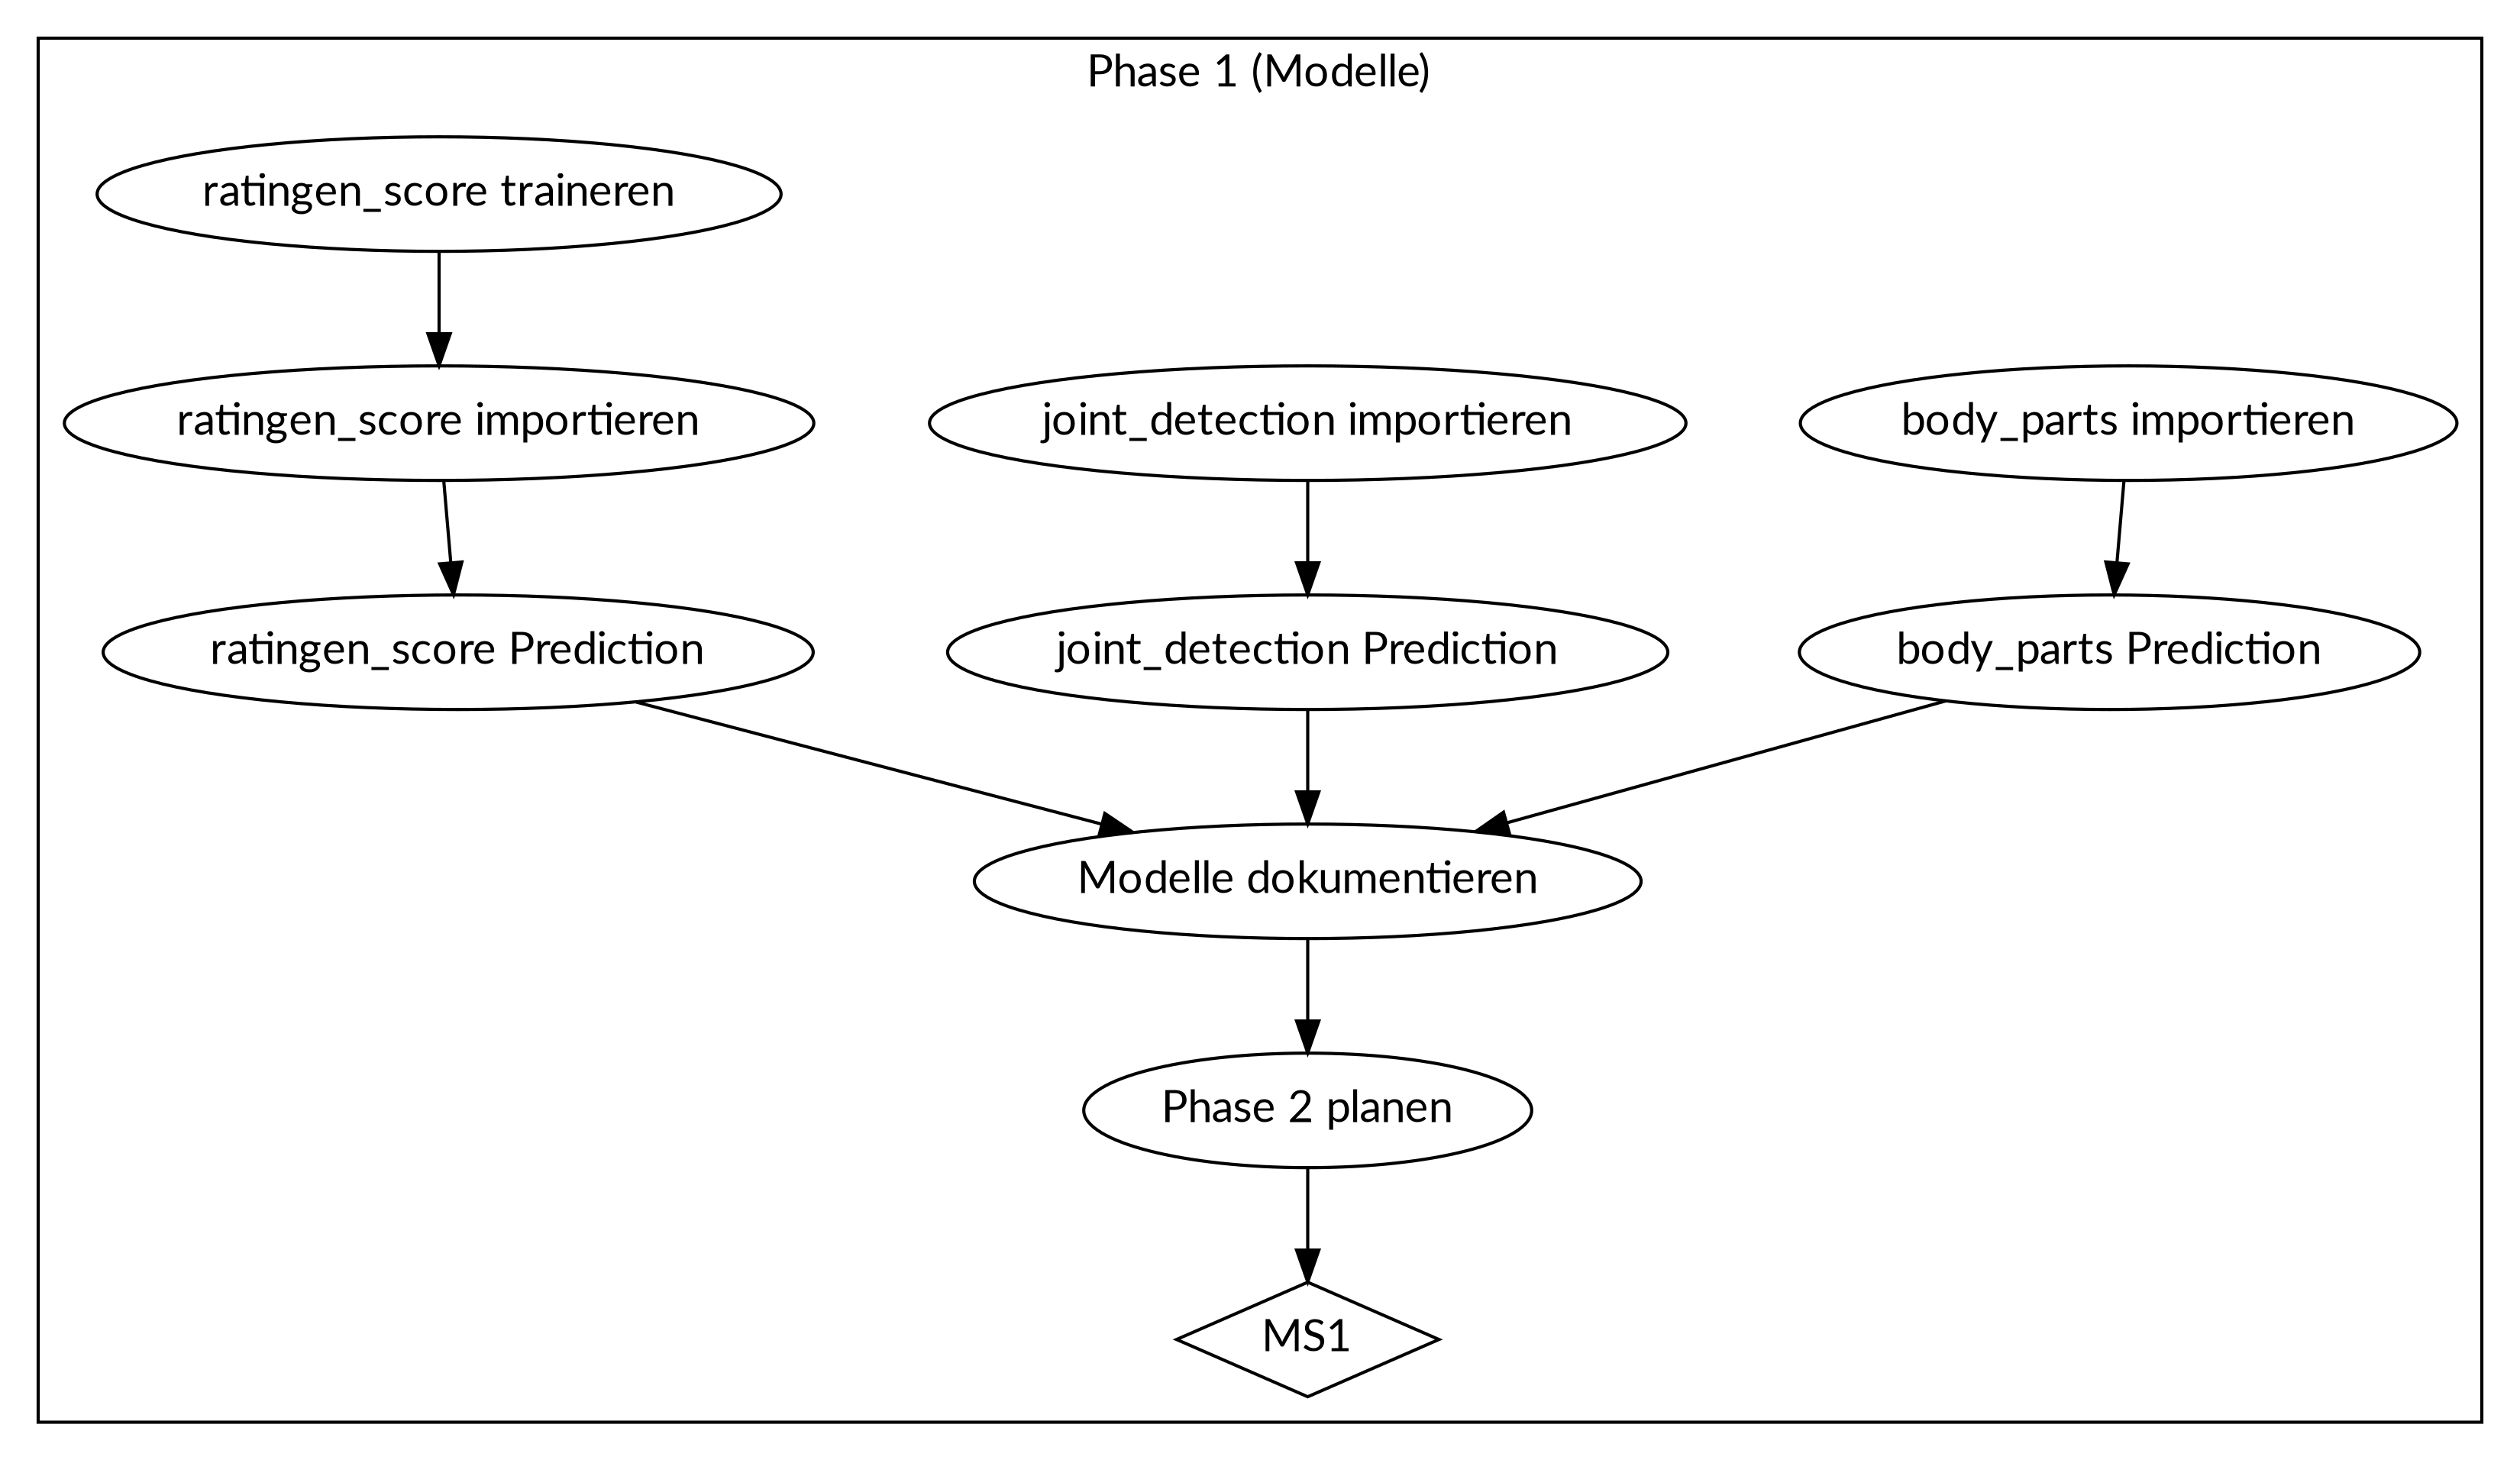
\includegraphics[width=\linewidth]{pics/phase1.png}
    \caption{In der ersten Projektphase werden die drei Modelle lauffähig gemacht und dokumentiert.}
    \label{fig:projekt-phase1}
\end{figure}

\paragraph{Reflexion}

Das Modell \texttt{ratingen\_score} konnte neu trainiert und erfolgreich exportiert werden. Alle drei Modelle sind in einer isolierten Umgebung (Docker-Container) lauffähig. Die Predictions der Modelle sind plausibel, wobei hierfür keine systematischen Tests vorgenommen worden sind. Die Laufzeitperformance erscheint als akzeptabel; die Predictions laufen in Sekundenschnelle ab.

\subsubsection{Zweite Phase: Architektur}

\begin{itemize}
    \item \textbf{Ziel:} Architektur und Evaluationsmetriken festlegen
    \item \textbf{Artefakte}
        \begin{enumerate}
            \item Architekturvorschläge und -diskussion
            \item begründeter Architekturentscheid
            \item Liste mit einzusetzenden Technologien
            \item Evaluationsmetriken
            \item Testkonzept
            \item Planung Phase 3
        \end{enumerate}
    \item \textbf{Aufgaben}
        \begin{enumerate}
            \item Architektur
                \begin{multicols}{2}
                    \begin{enumerate}
                        \item Integrationsvarianten finden
                        \item Architekturvorschläge aufstellen
                        \item Architekturvariante auswählen
                        \item Technologien finden
                        \item Prototyp implementieren
                    \end{enumerate}
                \end{multicols}
            \item Evaluation
                \begin{multicols}{2}
                    \begin{enumerate}
                        \item Datentypen finden
                        \item Datentypen der Modelle ermitteln
                        \item Evaluationsmetriken finden
                        \item Evaluationsmetriken bewerten
                        \item Geeignete Evaluationsmetriken auswählen
                    \end{enumerate}
                \end{multicols}
        \end{enumerate}
    \item \textbf{Risiken und Mitigationen}
        \begin{enumerate}
            \item Es lassen sich keine geeigneten Technologien für einen Architekturvorschlag finden.
                \begin{enumerate}
                    \item Es wird auf eine andere Architekturvariante ausgewichen.
                \end{enumerate}
            \item Der Prototyp kann mit der vorgeschlagenen Architekturvariante nicht umgesetzt werden.
                \begin{enumerate}
                    \item Es wird auf eine andere Architekturvariante ausgewichen.
                    \item Ein weiterer Prototyp wird implementiert, um die andere Variante zu prüfen.
                \end{enumerate}
            \item Es gibt keine geeigneten Evaluationsmetriken für das Gesamtsystem.
                \begin{enumerate}
                    \item Die Evaluation wird isoliert für die einzelnen Modelle vorgenommen.
                \end{enumerate}
        \end{enumerate}
\end{itemize}

\begin{figure}
    \centering
    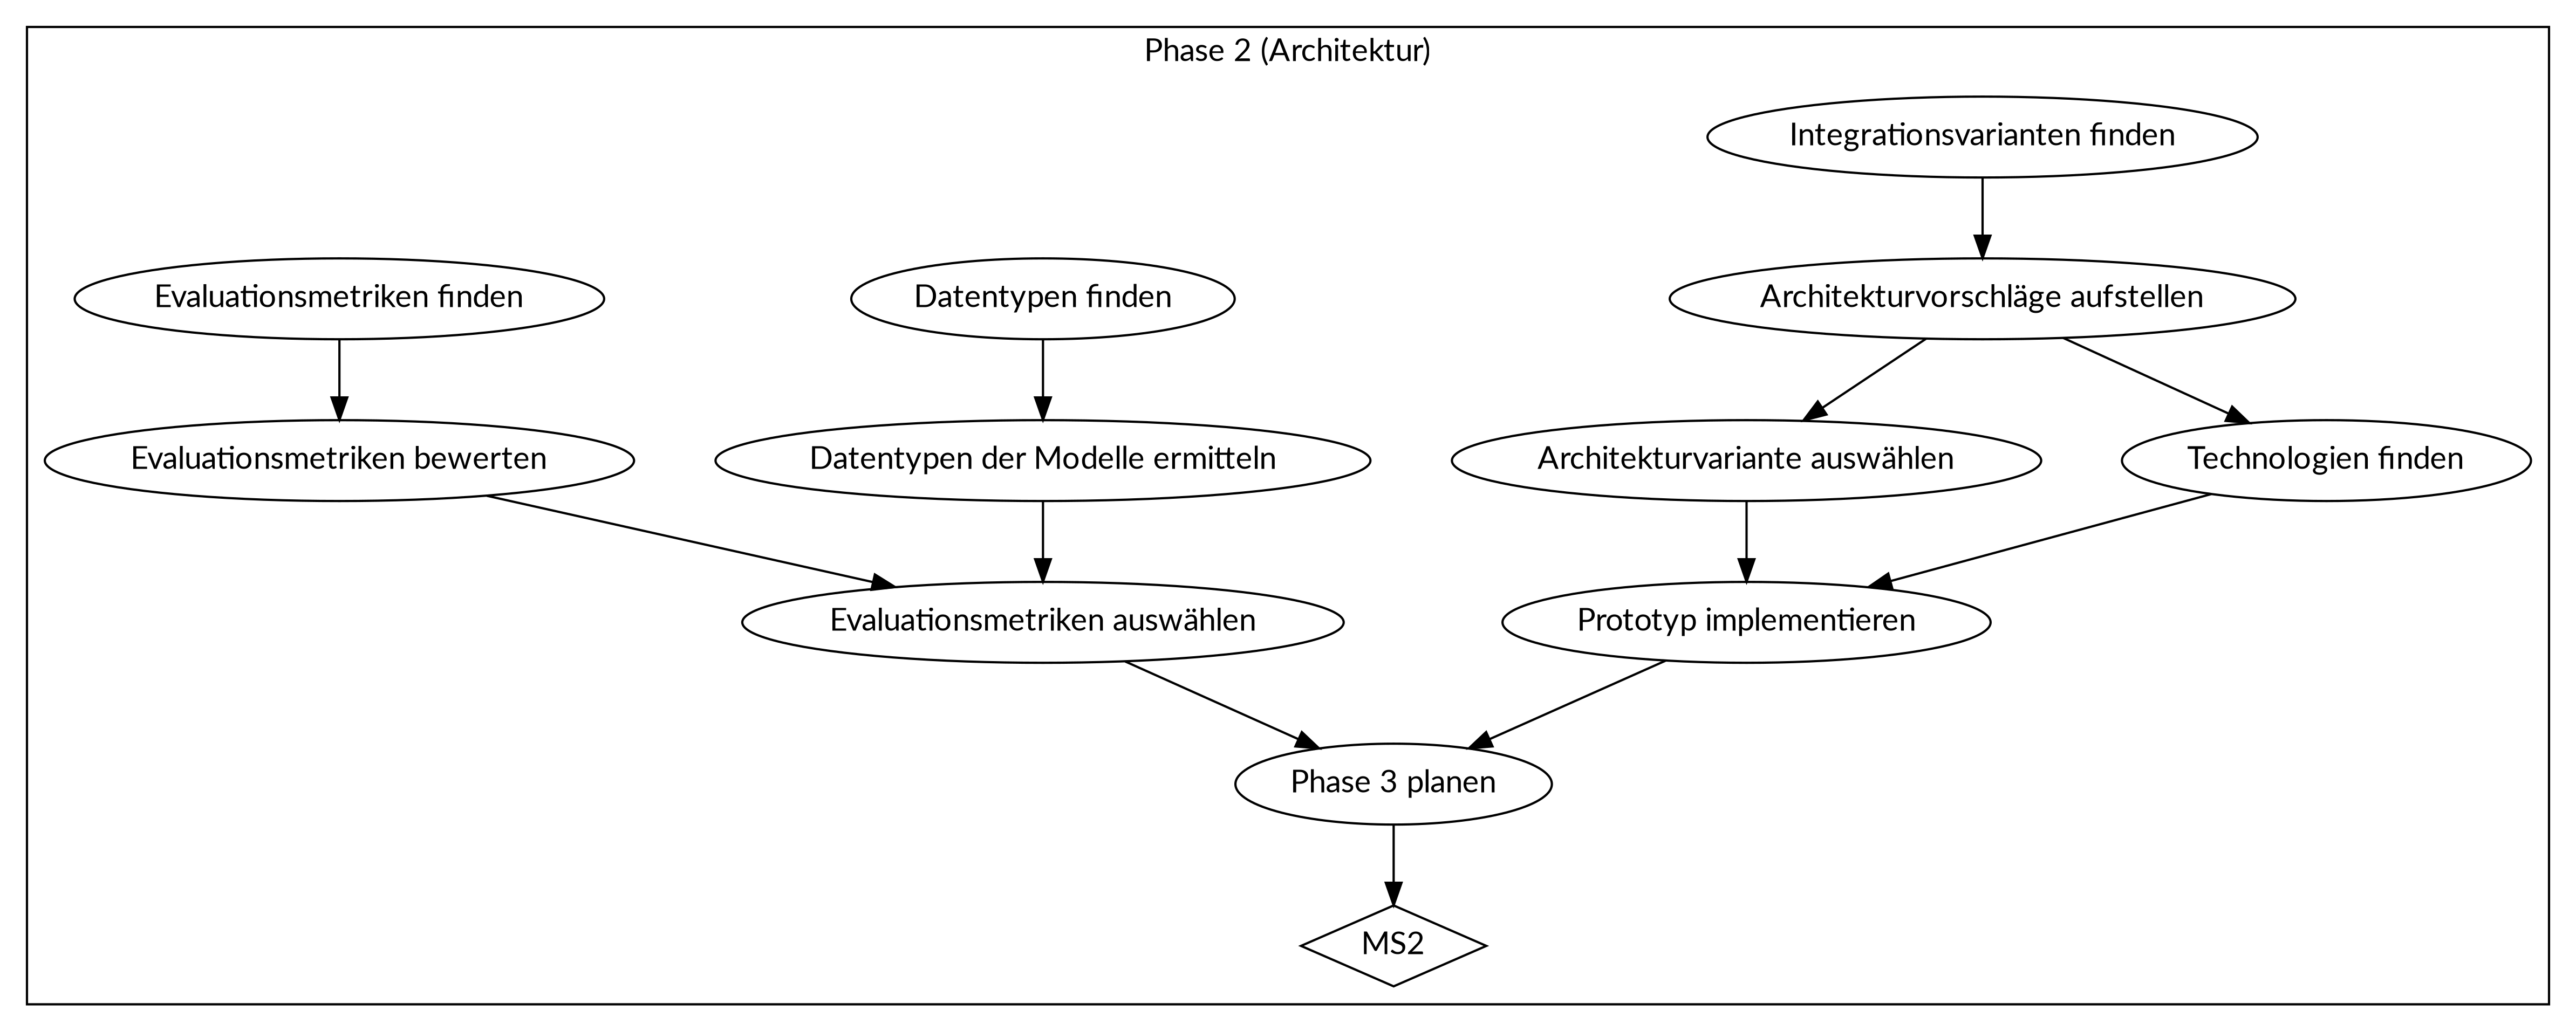
\includegraphics[width=\linewidth]{pics/phase2.png}
    \caption{In der zweiten Projektphase sollen Architekturvarianten und Evaluationsmetriken gefunden werden. Mithilfe eines Prototyps wird der Architekturvorschlag validiert.}
    \label{fig:projekt-phase2}
\end{figure}

\paragraph{Reflexion}

Das Auffinden verschiedener Integrationsvarianten, dazu passender Technologien und Evaluationsmetriken gestaltete sich sehr einfach. Hier war eher die Vielzahl der Möglichkeiten als deren Mangel ein Problem. Die Ausgestaltung und Auswahl der Architekturvarianten hat sehr viel Zeit in Anspruch genommen. Diese Investition hat sich jedoch gelohnt, zumal der Prototyp auf Anhieb funktioniert hat und als Vorlage für den zu erstellenden Webservice dienen kann.

\subsubsection{Dritte Phase: Orchestrierung}


\begin{itemize}
    \item \textbf{Ziel:} lauffähiger Prototyp mit Evaluationsergebnissen
    \item \textbf{Artefakte}
        \begin{enumerate}
            \item ausführbarer Programmcode
            \item ausführbare Testfälle
            \item gelabelte Evaluationsdaten
            \item Evaluationsworkflow (Programmcode)
            \item Evaluationsergebnisse
        \end{enumerate}
    \item \textbf{Aufgaben}
        \begin{enumerate}
            \item Webservice-Prototyp
                \begin{multicols}{2}
                    \begin{enumerate}
                        \item \texttt{body\_part} umsetzen
                        \item \texttt{joint\_detection} umsetzen
                        \item \texttt{ratingen\_score} umsetzen
                        \item \texttt{orchestrator} umsetzen
                        \item Web-UI umsetzen
                    \end{enumerate}
                \end{multicols}
            \item Evaluation
                \begin{multicols}{2}
                    \begin{enumerate}
                        \item Evaluationsdaten selektieren
                        \item Evaluationsdaten aufbereiten
                        \item Evaluationsdaten scoren
                        \item Evaluationsworkflow umsetzen
                        \item Ergebnisse evaluieren
                    \end{enumerate}
                \end{multicols}
        \end{enumerate}
    \item \textbf{Risiken und Mitigationen}
        \begin{enumerate}
            \item Der Webservice läuft zu langsam.
                \begin{enumerate}
                    \item Es soll eine performantere Laufzeitumgebung verwendet werden.
                    \item Die geringe Performance soll analysiert, Verbesserungsvorschläge sollen im Ausblick dokumentiert werden.
                \end{enumerate}
            \item Die asynchrone Architektur führt zu inkonsistenten Ergebnissen (Vermischung der Resultate).
                \begin{enumerate}
                    \item Es sollen zuverlässige Synchronisationsmassnahmen eingesetzt werden.
                    \item Es kann auf eine synchrone Architektur ausgewichen werden.
                \end{enumerate}
            \item Es stehen keine oder zu wenige Evaluationsdaten zur Verfügung.
                \begin{enumerate}
                    \item Der Evaluationsworkflow wird nur mit Platzhalterdaten ausgeführt. Die Evaluationsergebnisse sollen zu einem späteren Zeitpunkt vom Auftraggeber ermittelt werden.
                \end{enumerate}
            \item Die Evaluationsdaten lassen sich nicht in nützlicher Frist verarbeiten.
                \begin{enumerate}
                    \item Es soll nur eine Untermenge der Evaluationsdaten verarbeitet werden.
                \end{enumerate}
            \item Die Evaluationsergebnisse sind unbefriedigend (schlechte Performance).
                \begin{enumerate}
                    \item Dieses Risiko ist für den Auftraggeber zu tragen, da die Modelle (und somit die Prediction-Performance) vorgegeben waren.
                \end{enumerate}
        \end{enumerate}
\end{itemize}

\begin{figure}[tbh]
    \centering
    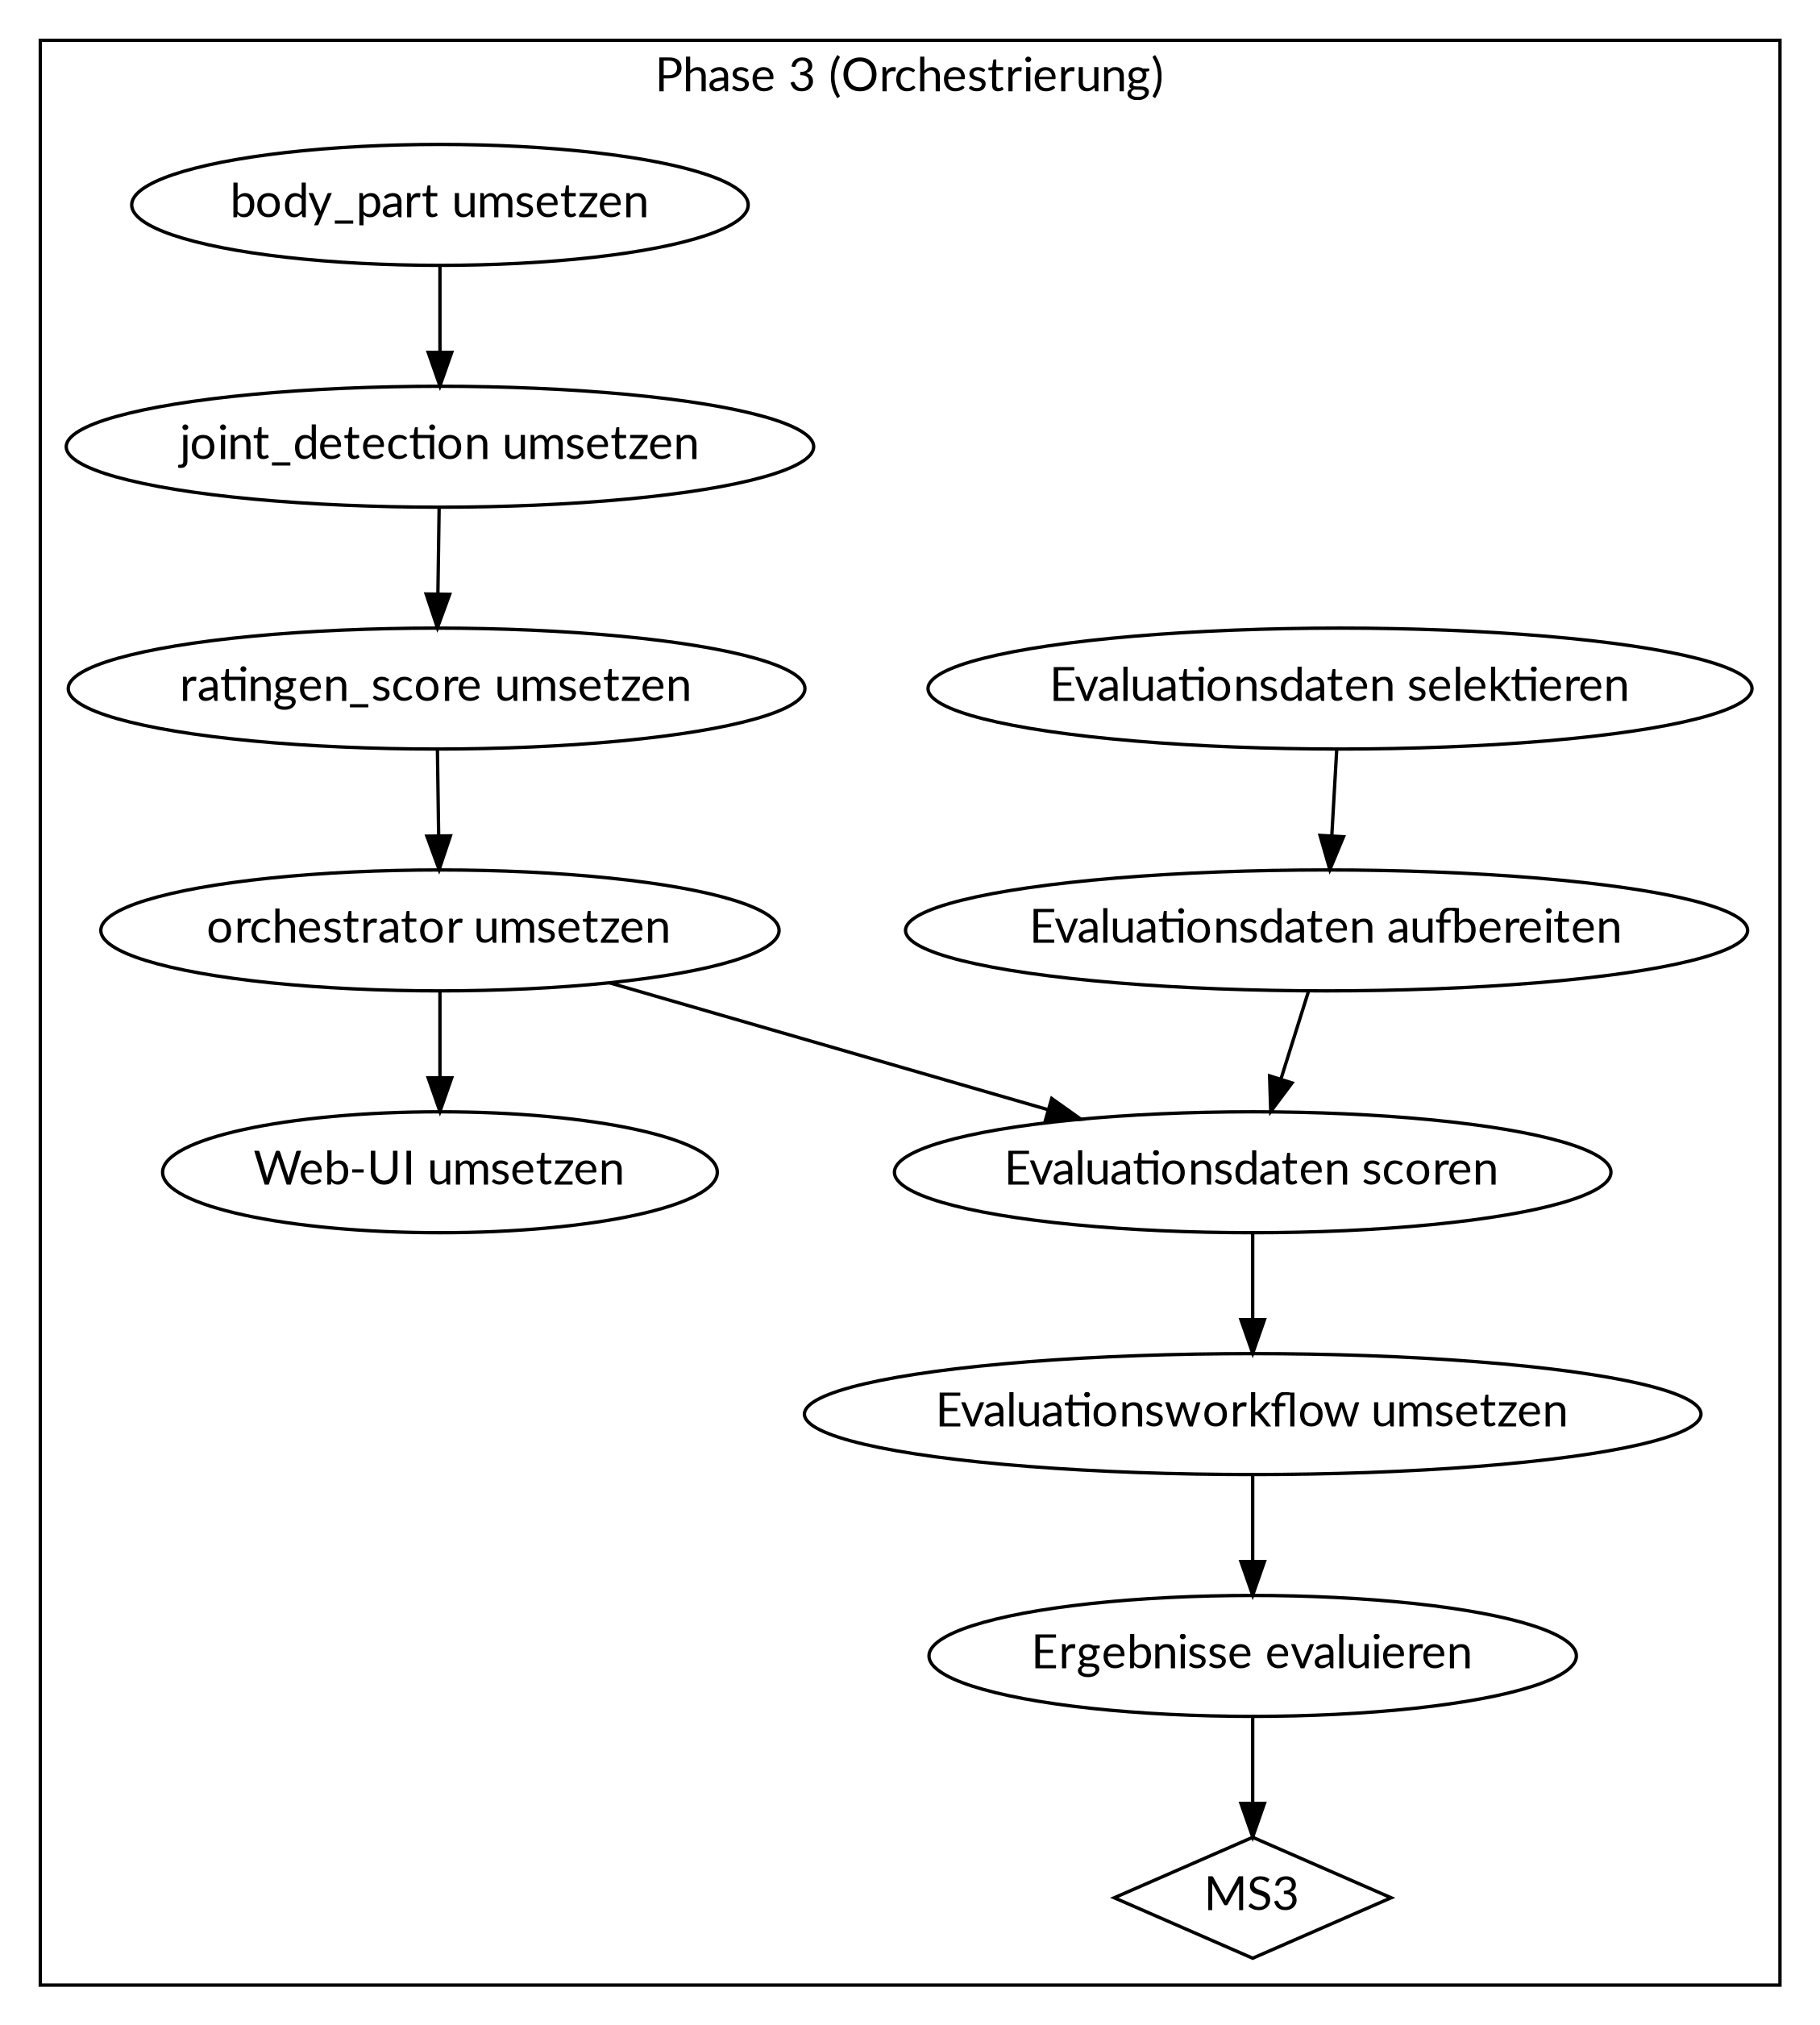
\includegraphics[width=0.7\linewidth]{pics/phase3.png}
    \caption{In der dritten Projektphase werden die einzelnen Teile zu einem lauffähigen System kombiniert. Dieses wird mit ausgewählten Metriken und entsprechenden Daten evaluiert.}
    \label{fig:projekt-phase3}
\end{figure}

\paragraph{Reflexion}

Der Prototyp aus Phase 2 hat sich als Glücksfall erwiesen, zumal der Webservice analog zu ihm umgesetzt werden konnte. Mit den gewählten Technologien (Go, RabbitMQ, Docker) konnte der Webservice erstaunlich schnell umgesetzt werden ‒ und lässt sich ohne Änderungen auf verschiedenen Umgebungen ausführen. Die Laufzeitperformance des Gesamtsystems ist für einen Prototyp akzeptabel, für den Produktiveinsatz jedoch verbesserungswürdig. Es konnten (in teilweise manueller Arbeit) genügend Evaluationsdaten gesammelt werden, um damit den Evaluationsworkflow umzusetzen und angemessen auf Plausibilität testen zu können. Für eine aussagekräftige Evaluation wären jedoch noch weitere ungesehene Daten nötig.

\subsubsection{Meilensteinplanung}

Die Meilensteinplanung (siehe \tblref{tbl:meilensteinplanung}) deckt sich grösstenteils mit der Projektphasenplanung, zumal am Ende einer jeden Projektphase ein Meilenstein erreicht werden soll. Als vierter und entscheidender Meilenstein kommt die Schlussabgabe hinzu, bei der zusätzlich die Artefakte Bericht, Web-Abstract und Pitching-Video abzuliefern sind.

\begin{table}[tbh]
    \center
    \small{
        \begin{tabular}{r|r|l|l}
            MS & SW & Datum & Beschreibung \\ \hline
            1 & 6 & 31.03.2020 & Phase 1 (Modelle) abgeschlossen \\
            2 & 8 & 19.04.2020 & Phase 2 (Architektur) abgeschlossen \\
            3 & 13 & 24.05.2020 & Phase 3 (Orchestrierung) abgeschlossen \\
            4 & 15 & 05.06.2020 & Schlussabgabe \\
        \end{tabular}
    }
    \caption{In der Meilensteinplanung wird neben den drei detailliert geplanten Projektphasen auch die Schlussabgabe als vierter Meilenstein berücksichtigt.}
    \label{tbl:meilensteinplanung}
\end{table}

\subsubsection{Wochenplan}

Obwohl in der Projektplanung (siehe \secref{sec:projektphasen}) auf eine detaillierte zeitliche Planung der einzelnen Aufgaben innerhalb der verschiedenen Projektphasen verzichtet worden ist, soll der Wochenplan (siehe \tblref{tbl:wochenplanung}) eine zusätzliche zeitliche Orientierung ermöglichen. Im Gegensatz zum Meilensteinplan ist im Wochenplan auch die Erstellung der Schlusspräsentation berücksichtigt, welche in den Wochen nach der Abgabe erfolgen soll.

\begin{table}[tbh]
    \small{
        \begin{tabularx}{\textwidth}{r|r|r|X|X}
            SW & Von & Bis & Tätigkeiten & Ereignis/Meilenstein \\ \hline
            0 & 12.02. & 16.02. & Projektinitialisierung (Kick-Off) & Projektstart \\
            1 & 17.02. & 23.02. & Recherche, Bestandesaufnahme & \\
            2 & 24.02. & 01.03. & Recherche, Import bestehender Modelle & \\
            3 & 02.03. & 08.03. & Recherche, Import bestehender Modelle & \\
            4 & 09.03. & 15.03. & Recherche, Projektplanung & Erteilung def. Projektauftrag \\
            5 & 16.03. & 22.03. & Import/Ausführung bestehender Modelle & \\
            6 & 23.03. & 29.03. & Import/Ausführung bestehender Modelle, Dokumentation & \\
            7 & 30.03. & 05.04. & Dokumentation, Planung, Architektur & MS1 \\
            8 & 06.04. & 12.04. & Architektur & \\
            9 & 13.04. & 19.04. & Architektur, Dokumentation, Planung & MS2 \\
            10 & 20.04. & 26.04. & Umsetzung, Dokumentation & Zwischenpräsentation \\
            11 & 27.04. & 03.05. & Umsetzung, Dokumentation & \\
            12 & 04.05. & 10.05. & Umsetzung, Dokumentation & \\
            13 & 11.05. & 17.05. & Umsetzung, Dokumentation & \\
            14 & 18.05. & 24.05. & Deployment, Dokumentation & MS3, lauffähiger Prototyp \\
            15 & 25.05. & 31.05. & Dokumentation, Video & \\
            16 & 01.06. & 05.06. & Abschliessen Dokumentation & Schlussabgabe \\
            & 06.05. & 30.06. & Abschlusspräsentation erstellen & Abschlusspräsentation \\
        \end{tabularx}
    }
    \caption{Der Wochenplan dient ‒ als Ergänzung zu Phasen- und Meilensteinplan ‒ als zeitliche Orientierungshilfe für den Projektablauf.}
    \label{tbl:wochenplanung}
\end{table}

\clearpage

\subsection{Teststrategie}
\label{sec:teststrategie}

Wie bereits im Modul \textit{Software Testing} (Frühlingssemester 2019) eingeübt und im \textit{Wirtschaftsprojekt} (Herbstsemester 2019) gewinnbringend eingesetzt, sollen die \textit{Agile Test Quadrants} (\imgref{fig:agile-testing-quadrants}) wiederum als Grundlage für die Erarbeitung einer Teststrategie dienen.\footnote{Auf die Umsetzung der Tests wird erst im Folgekapitel \secref{sec:realisierung} eingegangen.}

\begin{figure}[tbh]
    \centering
    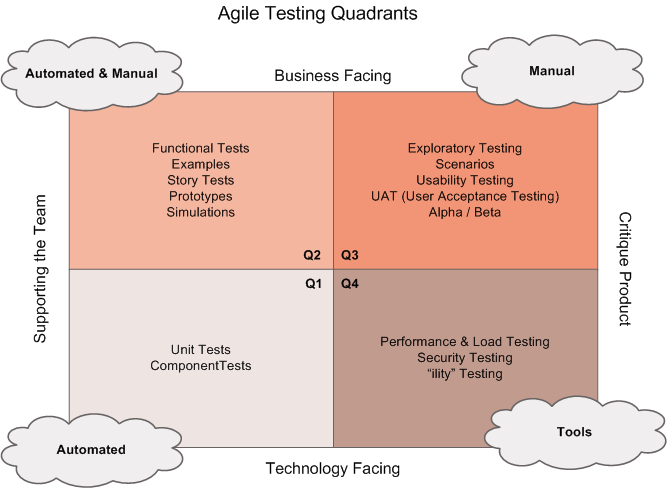
\includegraphics[width=\linewidth]{pics/agile-testing-quadrants.png}
    \caption{Die \textit{Agile Testing Quadrants} (\url{https://lisacrispin.com/2011/11/08/using-the-agile-testing-quadrants}) sind eine bewährte Orientierungshilfe für das Erarbeiten einer Teststrategie.}
    \label{fig:agile-testing-quadrants}
\end{figure}

Die verschiedenen Arten von Tests werden dabei als Werkzeuge betrachtet, die man für geeignete Aufgaben einsetzt ‒ und für weniger geeignete Aufgaben wieder in die Werkzeugkiste zurücklegt. Die Wahl der Testwerkzeuge soll pragmatisch erfolgen, d.h. im Hinblick auf ihre Effektivität (ein Systemmerkmal wird sinnvoll geprüft) und Effizienz (mit wenig Testcode kann viel produktiver Code abgedeckt werden). Eindimensionale Metriken wie \textit{«Es soll 95\% des Codes mit Unittests abgedeckt werden»} lesen sich bei diesem Verständnis wie \textit{«Der Bau der Hundehütte soll weitgehendst mit dem Hammer erfolgen»}. \footnote{Mit den Einfluss der Werkzeuge auf das Denken hat sich u.a. Edsger W. Dijkstra befasst \cite{dijkstra-council}. Das Zitat, \textit{«If your only tool is a hammer, then every problem looks like a nail.»}, dessen Ursprung umstritten ist \cite{quoteinvestigator}, veranschaulicht das Problem pointiert.} 

Die vier Quadranten, und ihre möglichen Anwendungen für das vorliegende Projekt \textit{DeepXRay}, werden im Folgenden beschrieben.

\subsubsection{Q1: automatisiert}

Im ersten Quadranten geht es um Unittests und Komponententests. Diese sollen v.a. für den neu zu erstellenden Code geschrieben werden, der keine Abhängigkeit zu anderen Laufzeitkomponenten hat. Beim bestehenden Code (Modelle) ist dies nur teilweise sinnvoll, zumal es sich dabei um Legacy-Code handelt, der eher abgelöst als erweitert werden soll. Beim \texttt{orchestrator}, der viele Abhängigkeiten zu anderen Laufzeitkomponenten hat, wären solche Tests nur über umfassendes und aufwändiges \textit{Mocking} möglich.\footnote{Beim Mocking wird häufig die interne Funktionsweise des Testcodes simuliert. Hierzu ist nicht nur Kenntnis der Schnittstelle, sondern auch der Implementierung vonnöten. Unittests, die Mocking verwenden, sind daher häufig fragil ‒ und strenggenommen keine Black-Box-Tests. Mocking, bzw. dessen Notwendigkeit für das Schreiben von Unittests, gilt daher teilweise als \textit{Code Smell} \cite[S. 214]{composing-software}.} Der Evaluationsworkflow hingegen, bei dem verschiedene mathematische Metriken implementiert werden müssen, lässt sich hervorragend mittels Unittests prüfen.

Für den Evaluationscode soll auch die Testabdeckung gemessen werden. Absolute Ziele (z.B. \textit{«95\% der Codezeilen durch Testfälle abgedeckt»}) sind dabei wenig hilfreich, da man eine hohe Codeabdeckung auch erreichen kann, ohne die Ergebnisse zu überprüfen, die vom jeweiligen Code zurückgeliefert werden. Vielmehr geht es beim Messen der Testabdeckung darum, auf Codepassagen aufmerksam zu werden, die nicht automatisiert getestet werden.

\subsubsection{Q2: automatisiert und manuell}

Im zweiten Quadranten geht es um Tests, die manuell durchgeführt, bei Bedarf aber auch automatisiert werden können.

Das Vorgehen im Wirtschaftsprojekt im letzten Herbst hat sich dabei als sehr sinnvoll erwiesen: Tests werden zunächst manuell durchgeführt. Erst wenn man bemerkt, dass ein und derselbe Test immer wieder durchgeführt werden muss ‒ und das Testen die Hände stärker beansprucht als den Kopf ‒, wird der Test mithilfe eines Testskripts automatisiert. So leistet man nur dort Automatisierungsarbeit, wo diese wirklich sinnvoll ist.

Im vorliegenden Projekt könnten folgende Arten von Tests sinnvollerweise automatisiert werden:

\begin{description}
    \item[Tests der einzelnen Modelle] Da die Erstellung der Modelle nicht Bestandteil der Arbeit ist, werden die Modelle nicht auf Performance im Sinne «korrekter» Predictions geprüft. Es geht vielmehr darum zu prüfen, ob das Modell auch von aussen ansprechbar ist und soweit «korrekt» arbeitet, wie es eben erstellt worden ist. Hierzu können Sammlungen von Testdaten erstellt werden, die Inputs zu Outputs mappen. Dies könnte etwa folgendermassen aussehen:
        \begin{itemize}
            \item \texttt{body\_part}: Ein Bild (Input) wird zu einem String (erkanntes Körperteil) gemappt.
            \item \texttt{joint\_detection}: Ein Bild (Input) wird zu zehn anderen Bildern (extrahierte Gelenke) ‒ oder zu einer Fehlermeldung, falls keine Gelenke erkannt worden sind, ‒ gemappt.
            \item \texttt{ratingen\_score}: Ein kleines Bild von einem Gelenk, das aus einer Röntgenaufnahme extrahiert worden ist, wird zu einer Score gemappt.
        \end{itemize}
    \item[Tests über das ganze System] Hierbei können die Testdefinitionen der einzelnen Modelle wiederverwendet werden, indem etwa ein ganzes Röntgenbild (Input) zu einer Reihe von Scores (oder zu einer Fehlermeldung) gemappt wird.
\end{description}

Für diese Testdefinitionen ist ein sinnvolles Format zu definieren. Eine Möglichkeit wäre JSON-Dateien, die einen Dateinamen zu einem Output mappen. Diese JSON-Dateien könnten statt Dateinamen auch die eigentlichen Bilddaten enthalten, indem diese base64-kodiert direkt eingefügt werden. Beim ersten Ansatz wird das manuelle Betrachten von Testinputs einfacher. Im zweiten Ansatz sind die Testdaten schöner abgekapselt.

In jedem Fall muss ein Testrunner entwickelt werden, der mit den definierten Testdaten umgehen kann. Je nach verwendeter Schnittstelle sieht ein solcher Testrunner anders aus. Mit dem Python-Testframework PyTest und der Testing-Library von Go konnten dabei schon viele positive Erfahrungen gesammelt werden.

Um die nebenläufige Verarbeitung von Röntgenbildern testen zu können, soll ein (nicht-deterministischer) Testfall erstellt werden, der mehrere Röntgenbilder schnell nacheinander zur Verarbeitung übergibt, ohne die eintreffenden Antworten synchron abzuwarten. Diese werden nebenläufig eingesammelt. Die Antworten sind darauf zu prüfen, dass sie immer die gleichen Scores pro Röntgenbild enthalten. So kann (mit hoher Wahrscheinlichkeit) sichergestellt werden, dass der \texttt{orchestrator} die einzelnen Vorgänge intern korrekt auseinanderhält.

\subsubsection{Q3: manuell}

Der dritte Quadrant spielt im Rahmen der vorliegenden Arbeit nur eine sehr untergeordnete Rolle. Da die grafische Benutzeroberfläche, die für den Prototyp erstellt wird, nur zu Demozwecken dienen soll und kein eigentliches Lieferobjekt des vorliegenden Projekts ist, erübrigen sich formalisierte Tests desselben.

Manuelle Tests könnten sich aber an andere Stakeholder richten und sich auf die Umgebung des Prototyps beziehen.

\begin{itemize}
    \item Wie kann die Umgebung in Betrieb genommen werden?
    \item Wie können die Testfälle ausgeführt werden?
    \item Wie finde ich Hilfe (Dokumentation), wenn etwas nicht (mehr) funktioniert?
\end{itemize}

Rückmeldungen in diesem Bereich sind gerade im Hinblick auf die Abgabe des Projekts sinnvoll, und könnten vom Auftraggeber und vom Betreuer eingeholt werden.

\subsubsection{Q4: Tools}

Im vierten Quadranten geht es v.a. um das Testen nicht-funktionaler Anforderungen, d.h. Performance, Security, Usability usw. Da es im vorliegenden Projekt nur um die Entwicklung eines Prototyps geht, können Überlegungen zu den Aspekten Security und Usability von Beginn weg weitgehend ausgeklammert worden.

Die Verarbeitung von Röntgenbildern kann mit einem Benchmark im Bezug auf die Laufzeitperformance untersucht werden. Go bietet hierfür passende Funktionalität in der Standardbibliothek \cite[Kapitel 11.4]{gopl}.

Flaschenhälse bei der Performance (CPU, Memory, I/O) könnten per Profiling ermittelt werden. Eine umfassende Analyse des Laufzeitverhaltens mittels Profiling ist jedoch aufwändig und soll nicht im Rahmen des vorliegenden Projekts erfolgen.

Für die Codequalität ist es sinnvoll, wenn statische Codeanalyse verwendet wird. Sogenannte Linter führen auf Basis von Regeln und Heuristiken Codeüberprüfungen durch und geben Warnungen bei potenziellen Problemen ab, die meist stilistischer Natur sind. Mögliche Werkzeute sind \texttt{pylint} (Python) und \texttt{golint} (Go). Code-Auditing-Tools wie \texttt{py\-lama} (Python) und \texttt{go vet} (Go) warnen den Programmierer vor möglichen Problemen und Fehlern, und sollten darum auch eingesetzt werden, idealerweise automatisiert und in der Entwicklungsumgebung integriert.

Bei der Verwendung von Tools ist es wichtig, dass diese einfach eingesetzt werden können. Im Wirtschaftsprojekt hat sich ein einfaches \texttt{Makefile} als gute Variante erwiesen. Mit Befehlen wie \texttt{make cover} wurden etwa alle Unittests ausgeführt und die Codeabdeckung ausgegeben. Müsste man den ganzen Befehl dafür jeweils von Hand eintippen oder in der Shell-History suchen, wäre der Aufruf entsprechend umständlicher.

\subsubsection{Testumgebung}

Wie der zu erstellende Prototyp sollen die Tests zunächst nur auf einer Test- bzw. Demoumgebung ausführbar sein. Bei Seantis wird die CI-Umgebung Buildkite\footnote{\url{https://buildkite.com/} (abgerufen am 17.05.2020)} verwendet, die sich nur mit grösserem Aufwand für neue Projekte einrichten lässt, zumal die erstellten Container für die Modellkomponenten dem CI-System über das interne Container-Buildtool \texttt{parts} zugänglich gemacht werden müssten.

Die Integration in die CI-Umgebung des Auftraggebers soll darum nicht Bestandteil des vorliegenden Projekts sein.
